\documentclass[sigconf]{acmart}

\usepackage{booktabs} % For formal tables
\usepackage{graphicx}
\usepackage{algorithm}  
\usepackage{algorithmicx}  
\usepackage{algpseudocode}  
\usepackage{amsmath}
\usepackage{url}
\usepackage{xcolor}
\usepackage{listings}
\usepackage{enumitem}

\algnewcommand{\LeftComment}[1]{\Statex \(\triangleright\) #1}

\renewcommand{\algorithmicrequire}{\textbf{Input:}}  
\renewcommand{\algorithmicensure}{\textbf{Output:}}  
\graphicspath{{figure/}}

% Copyright
%\setcopyright{none}
%\setcopyright{acmcopyright}
%\setcopyright{acmlicensed}
\setcopyright{rightsretained}
%\setcopyright{usgov}
%\setcopyright{usgovmixed}
%\setcopyright{cagov}
%\setcopyright{cagovmixed}

\settopmatter{printacmref=false}
\renewcommand\footnotetextcopyrightpermission[1]{} % removes footnote with conference information in first column
\pagestyle{plain}

% DOI
\acmDOI{10.475/123_4}

% ISBN
\acmISBN{123-4567-24-567/08/06}

%Conference
\acmConference[ICNNC]{2017 VI International Conference on Network, Communication and Computing}{2017}{China} 
\acmYear{2017}
\copyrightyear{2017}

\acmArticle{4}
\acmPrice{15.00}

\begin{document}
\title{Grouper: A Framework for Developing Mobile Applications using a Secret Sharing Scheme and Untrusted Servers}

\author{Meng Li}
\affiliation{University of Tsukuba}
\email{limeng@softlab.cs.tsukuba.ac.jp}

\author{Yasushi Shinjo}
\affiliation{University of Tsukuba}
\email{yas@cs.tsukuba.ac.jp}

% The default list of authors is too long for headers.
\renewcommand{\shortauthors}{Li et al.}

\begin{abstract}
	
Conventional mobile applications are built based on a client-server modal and require central servers for storing shared data and processing confidential information.
If the central servers are accessed by an attacker, a curious administrator or a government, private information will be revealed because data is often stored on the central servers in the form of cleartext.
This paper presents Grouper, a framework for developing mobile applications without trusted central servers.
Grouper provides object synchronization among mobile devices.
It also uses a secret sharing scheme to create several shares from a marshalled object and uploads these shares to multiple untrusted servers. 
These untrusted servers construct a self-destruction system.
Uploaded shares will be deleted after a certain period of time.
Mobile devices exchange messages via untrusted servers based on the Grouper Message Protocol.
Grouper consists of a client framework and a Web service.
We have implemented client framework for iOS, macOS, tvOS and watchOS in Objective-C.
The Web service is implemented in Java and runs on multiple untrusted servers.
We have implemented two applications using Grouper: an iOS application named Account Book, and a benchmark application named Test.
We have evaluated the development efforts associated with implementing Grouper as well as its and the performance. 
Developing these applications demonstrates that Grouper requires little development effort to convert a standalone application to a data sharing application.
Experimental results prove that the performance of Grouper is satisfactory for mobile applications that are used among a small group of people.

\end{abstract}

\keywords{Mobile application security; secret sharing; untrusted server}

\maketitle

\section{Introduction}

People use mobile applications every day. 
Conventional mobile applications are built based on a client-server mode and require central servers for storing shared data and processing confidential information.
When users use mobile applications, users fully trust the central servers.
In fact, they are often unaware of their existence and simply rely on the functionality to be provided.
If the central servers are accessed by an attacker, a curious administrator or a government, private information will be revealed because data is often stored on the central servers in the form of cleartext.
In addition, users may lose their data when service providers shut their servers down.

To address the problem of using central servers, Vanish\cite{geambasu2009vanish}, SafeVanish\cite{zeng2010safevanish}, SeDas\cite{zeng2012sedas} and CouldSky\cite{zeng2015cloudsky} constructed a data self-destruction system as their cloud storage.
In these approaches, servers store encrypted data temporarily and delete it after a certain period of time.

These existing approaches have several problems.
First, they do not support data recovery when some nodes are unable to obtain data from shared storage.
Often, application developers have to deal with such cases on their own.
Second, these approaches do not support developing general mobile applications.

To address these problems, we are developing Grouper, a framework for developing mobile applications. 
Grouper provides object synchronization among mobile devices.
In Grouper, a sender node translates an updated object into shares using a secret sharing scheme and uploads these shares to untrusted servers. 
A receiver node downloads some of these shares and reconstructs the object.
The untrusted servers construct a self-destruction system, and delete these shares after a period of time.
Unlike existing approaches, Grouper supports data recovery when some nodes are unable to obtain shares from untrusted servers.
When a receiver node is unable to obtain shares, the Grouper framework automatically asks the sender to upload the missing shares again.
This ensures reliable data sharing among the devices of a group.
In addition, data can be recovered even if untrusted servers shut down because all devices of a group have the complete data set of this group.

Grouper consists of a client framework and a Web service.
We have implemented the client framework for iOS, macOS, tvOS and watchOS in Objective-C.
The Web service is implemented in Java and runs on multiple untrusted servers.
We used a Sync\cite{sync} framework in Grouper to synchronize objects among mobile nodes.
We have implemented two applications using Grouper: an iOS application named Account Book, and a benchmark application named Test.
These implementations demonstrate that Grouper makes it easy to develop mobile applications with data synchronization.
Experimental results prove that the performance of Grouper is satisfactory for mobile applications that are used among a small group of people.

The contributions of this paper are as follows.
First, we provide support for data recovery when some nodes are unable to obtain data from untrusted servers.
Grouper provides reliable data synchronization among nodes using a reliable multicast technique.
Second, we make it easier to develop mobile applications.
In fact, a developer can add data synchronization functions to stand alone applications with a few lines of code.

\section{Threat Model}

In this section, we introduce the assumptions and the threat model underlying the Grouper framework.
We target mobile applications that are used among a small group of people.
A group consists of a special member called the owner and other members.
Each member has a mobile device.
The owner invites other members in a face-to-face manner.

First, because we use servers, they are passive adversaries and can read all of the data but they do not actively attack.
Servers host Web services and perform device authentication.
Servers generate access keys for group members. 
When a device wants to obtain/place data to/from servers, the device sends a request with an access key.
In this paper, we do not address other types of attacks such as user tracking and metadata collection by servers. 
For example, servers can track users with IP addresses, and Grouper cannot hide social graphs against such tracking.

Second, data transportation between a device and an untrusted server is secure.
We can protect it using Transport Layer Security (TLS) or other encryption techniques.
Grouper focuses on the privacy of the data storage on servers rather than on data transportation.

Third, in an application, all group members are not malicious and their devices connect to each other securely at a face-to-face distance at the time of user invitation.
For example, group members working in an office know on another and are not malicious.
When the group owner invites new members, the owner authenticates group members in a face-to-face manner.
Note that after user invitation, devices communicate through servers and no secure, direct communication path is required.

Last, servers are isolated from one another and managed by independent providers.
We assume that providers of untrusted servers do not expose user data to other providers.
For example, a group owner can leverage the servers of Amazon, Google, and Microsoft, which are not supposed to expose user data to other cloud providers.

\section{Design}

This section describes the design of the Grouper framework.

\subsection{Overview}

Our goal is to support the development of mobile applications that do not rely on trusted central servers.

To achieve this goal, we are developing the Grouper framework.
This framework provides the following functions:

\begin{itemize}
	\setlength{\itemsep}{1pt}
	\setlength{\parskip}{0pt}
	\setlength{\parsep}{0pt}
	\item \textbf{Data Synchronization.} 
	If an user updates or deletes an object in his device, the mirrors of this object in other devices are updated or deleted.
	\item \textbf{Group management.} 
	A group owner can create a group and invite other members to his group.
\end{itemize}

For example, \emph{Account Book} is an iOS application developed using Grouper. 
In this application, a leader of a small company can create a group and invite employees to join the group. 
Then, the employees can record the income and expenditure of their company.
These income and expenditure records are represented as objects and shared among devices.
Anyone can edit and delete existing records in his device.

Grouper uses untrusted servers to exchange messages among mobile devices.
Untrusted servers construct a self-destruction system, and delete messages after a certain period of time.
We refer to this as the Time to Live (TTL).

Grouper uses Shamir's secret sharing scheme to protect messages from the providers of untrusted servers.
In this scheme, a member securely shares a secret with other members by generating $n$ shares using a cryptographic function\cite{smith2013layered}. 
At least $k$ or more shares can reconstruct the secret, but $k-1$ or fewer shares output nothing about the secret\cite{pang2005new}. 
We describe this scheme as a function ${f(k, n)}$, where $n$ is the number of shares, and $k$ is the threshold to combine shares. 

Grouper has the following advantages over conventional approaches using a self-destruction system.
First, it is easy for a developer to recover from message losses in untrusted servers, as demonstrated in Section 3.4.
Grouper performs retransmission when some mobile devices miss getting messages from untrusted servers.
Developers of mobile applications do not have to specify the lifetimes of messages.
Second, it is easy for a group owner to invite other members using a safe communication channel at a face-to-face distance, as discussed in Section 3.7.

\subsection{Architecture}

\begin{table*}[t]
	\centering
	\small
	\caption{Client API of Grouper.}
	\begin{tabular}{ll}
		\hline
		\textbf{Method} & \textbf{Description} \\ \hline
		$grouper.\textbf{setup}(appId, dataStack)$ & 
		\begin{tabular}{@{}l@{}}
			An application invokes this method to initialize Grouper with appId and dataStack. AppId is the unique ID\\ of an application. Datastack is used by the synchronization plugin.
		\end{tabular}  \\ \hline
		$grouper.sender.\textbf{update}(object)$ & 
		\begin{tabular}{@{}l@{}}
			An application invokes this method after creating a new object or modifying an existing object. Grouper\\ performs updates asynchronously and sends an update message to other devices.
		\end{tabular} \\ \hline
		$grouper.sender.\textbf{delete}(object)$ & 
		\begin{tabular}{@{}l@{}}
			An application invokes this method when it wants to delete an existing object. Grouper will\\ delete the object and remove it from the persistent store of a device automatically, after sending a message to\\ other devices.
		\end{tabular} \\ \hline
		$grouper.receiver.\textbf{receive}(callback)$ & 
		\begin{tabular}{@{}l@{}}
			An applications invokes this method to register the callback function that is called after Grouper processes\\ the received messages and updates objects according to the messages. The application can use this\\ callback function to update the user screen. 
		\end{tabular} \\ \hline
		$grouper.sender.\textbf{confirm}()$ & 
		\begin{tabular}{@{}l@{}}
			An application needs to invoke this method periodically or occasionally to send a confirm message to other\\ devices.
		\end{tabular} \\ \hline
	\end{tabular}
\end{table*}

\begin{table*}[t]
	\centering
	\small
	\caption{API of the synchronization plugin.}
	\begin{tabular}{ll}
		\hline
		\textbf{Method} & \textbf{Description} \\ \hline
		$marshall(o)$ & Marshalls the object o and returns the marshalled byte array. \\
		$updateRemote(b)$ & Unmarshalls the byte array $b$ to the object and puts the object into the persistent store. \\ 
		$deleteRemote(b)$ & Deletes the object in the byte array $b$ of object IDs.\\ \hline
	\end{tabular}
\end{table*}

\begin{figure}[t]
	\centering
	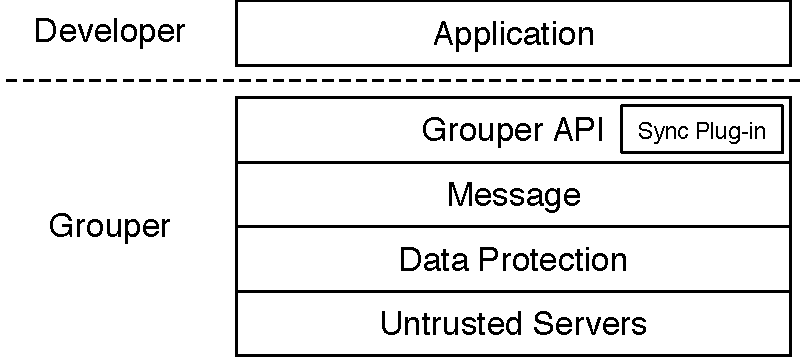
\includegraphics[scale=0.45]{architecture}
	\caption{Architecture of Grouper.}
\end{figure}

Figure 1 describes the architecture of the Grouper framework. 
Grouper consists of the following four layers and a plugin:

\begin{itemize}
	\setlength{\itemsep}{1pt}
	\setlength{\parskip}{0pt}
	\setlength{\parsep}{0pt}
	\item \textbf{Grouper API.}
	A developer develops an application without data synchronization at first. 
	He adds the synchronization function to his application by using the API.
	\item \textbf{Synchronization Plugin.} 
	Grouper uses third-party framework for data synchronization.
	This plugin marshalls an updated object in a local persistent store and the Grouper API layer passes the marshalled message to a lower message layer.
	When the Grouper API layer receives a message, this layer unmarshalls the message using the plugin, reconstructs the message, and puts the object included in the message into the persistent store.
	\item \textbf{Message.}
	This layer provides a messaging transportation service with multicasting capability among devices.
	The destination of a message is not only the node identifier (ID) of a single device, but also "*", which means it is delivered to all the other nodes.
	This layer does not ensure message delivery to other devices.
	\item \textbf{Data Protection.}
	Grouper protects user data by a secret sharing scheme in this layer.
	This layer divides a message into several shares, and uploads these shares to untrusted servers.
	When this layer downloads shares from untrusted servers, it recovers the original message using the secret sharing scheme.
	\item \textbf{Untrusted servers.}
	When a mobile device uploads a share to an untrusted server, this server receives it and stores it to a database.
	When a mobile device downloads a share from an untrusted server, this server retrieves it from the database and sends it into the device.
	An untrusted server performs device authentication using device keys.
\end{itemize}

The following subsections describe the details of these layers from the top layer to the bottom layer.

\subsection{Grouper API}

The Grouper framework provides object synchronization among mobile devices through a simple client API.
Table 1 shows the client APIs of Grouper that have been used to develop our target applications.
An application initializes the framework by invoking the method $grouper.setup()$.
When the application needs to update an object in all devices, the application invokes the method $grouper.sender.update()$.
When the application needs to delete an object in all devices, the application invokes the method $grouper.sender.delete()$.
The the application uses the method $grouper.receiver.receive()$ to register a callback function.
This callback function is called when another node updates an object and its local mirror has been updated.
The application can use this callback function to change the values that are shown on the user interface screen.
The method $grouper.confirm()$ is used for realizing reliable messaging.
We will describe reliable messaging in Section 3.4.

The Grouper API layer relies on the synchronization plugin.
As described in Table 2, the synchronization plugin should provide the functions $marshall(o)$, $updateRemote(b)$ and $deleteRemote(b)$.
Grouper invokes these functions to obtain marshalled data from the persistent store and save unmarshalled data in the persistent store.

We have not implemented the synchronization plugin on our own, but we provide it as a pluggable module.
This is because there are many such synchronization modules that provide various features.
Additionally, application requirements may also vary.
Each application developer should choose a suitable module based on a consistency model and other requirements.

Because we implement our client framework in Objective-C, we currently user the Sync framework\cite{sync} to implement the data synchronization plugin.
The Sync framework marshalls objects into JavaScript Object Notation (JSON) strings and provides a consistency model where the newest version wins.

\subsection{Reliable Message Delivery}

Grouper implements reliable message delivery in the Grouper API layer over the self-destruction system.

To design this, we use a reliable multicasting technique in distributed systems\cite{tanenbaum2007distributed}.
In this reliable multicasting technique, each message has a sequence number for each sender.
Each member keeps the newest sequence numbers for senders and detects missing messages.
If a member notices a missing message from a sender, the member asks the sender to resend the update message.
For example, consider that a sender sends update message No.3 to all other members using a multicast address.
When a member receives update message No.3, the member compares the sequence number 3 with the newest sequence number of the sender.
If the the newest sequence number of the sender is 1, this means the member missed update message No.2.
The member asks the sender to resend update message No.2 using a control message.
The sender will send update message No.2 to the the member who request it using a unicast address.

This basic reliable multicasting technique works well for continuous media, such as video streaming in Internet communication.
However, it does not work well if receivers go offline often or for a long time, as servers delete messages within a short time.

To address this problem, we extend the basic reliable multicasting technique.
We use a special type of message that includes active sequence numbers.
Using these messages, a receiver can easily identify missing messages.
We call these type of messages confirm messages.

\begin{figure}[t]
	\centering
	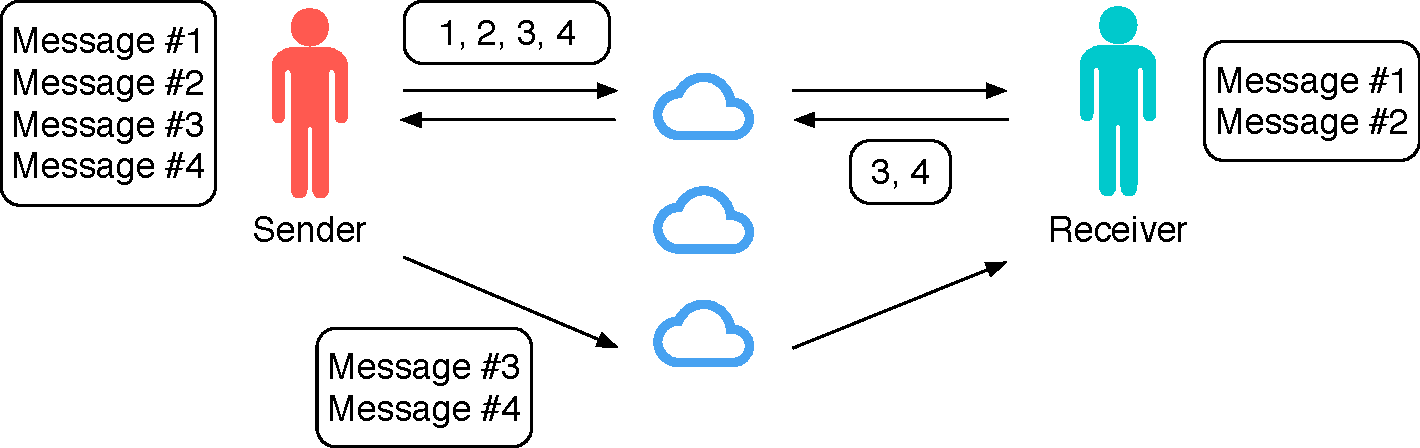
\includegraphics[scale=0.38]{reliable_sync}
	\caption{Implementing reliable messaging with continuous sequence numbers.}
\end{figure}

Figure 2 shows that the sender is sending five update messages, from No.1 to No.5, to the receiver.
The sender uploads two messages, No.1 and No.2, using a multicast address.
The receiver downloads these two messages and goes offline.
The servers delete these two messages.
The sender uploads the next three update messages, from No.3 to No.5, using a multicast address.
Again, the servers delete these three messages, again.
The receiver comes online, but the receiver does not notice that these three messages are missing.

At this time, the sender sends a confirm message that includes the newest active sequence number, 5, as shown in Figure 2.
The receiver receives this sequence number and compares it with the newest sequence number in the persistent store.
In Figure 2, the receiver notices that update messages No.3, No.4, and No.5 are missing.
The receiver asks the sender to resend update messages No.3, No.4, and No.5 using a resend message.
The sender will again send update messages No.3, No. 4, and No.5 to the receiver using a unicast address.

This idea is inspired by the checkgroups message of Usenet\cite{usenet}.
In Usenet, the list of active newsgroups is maintained with two basic messages: newgroup and rmgroup.
When a node receives a newgroup message, the node adds the newsgroup to the list.
When a node receives a rmgroup message, the node removes the newsgroup from the list.
However, these basic messages can be lost and the list can become obsolete.
Checkgroups messages supplement these basic messages.
A checkgroups message includes the list of all newsgroups in a newsgroup hierarchy.
A checkgroups message is distributed periodically or after some time after the basic messages are distributed.

\subsection{Data Protection}

The data protection layer uses Shamir's secret sharing scheme $f(k, n)$ as introduced in Section 3.1.
In Grouper, we extend this scheme and design a new scheme $ f(k, n, s)$.
In our scheme, the parameters $k$ and $n$ are same as those in the scheme $f(k, n)$. 
The parameter $s$ represents the minimum number of untrusted servers when a sender uploads shares, where $k \leq s \leq n$.
Although a receiver is able to recover the original message from at least $k$ shares, we should also consider the scenario in which the server crashes. 
When a sender has $n$ shares, Grouper tries to upload these $n$ shares to all $n$ untrusted servers, at first. 
If the shares are uploaded to $s$ or more untrusted servers, we consider that this upload to be successful.
Otherwise, Grouper continues trying to upload these shares.

Figure 3 shows the message transportation from a device to another device using the extended secret sharing scheme $f(2, 4, 3)$.
In this figure, the message layer in a sender device is sending a message to the message layer in a receiver device.
At first, this layer calls the data protection layer and creates four shares, according to the secret sharing scheme.
Next, this layer uploads those shares to four untrusted servers.
In Figure 3, although only the three untrusted servers on the left receives shares successfully, we regard this upload as successful.
Finally, the message layer in the receiver device downloads two shares from the four untrusted servers and recovers the message by calling the data protection layer.

We can choose the parameter $s$ based on the following policies.

\begin{itemize}
	\setlength{\itemsep}{1pt}
	\setlength{\parskip}{0pt}
	\setlength{\parsep}{0pt}
	\item \textbf{Sender first.} 
	An application sets $s$ closed to $k$. 
	A sender receives a successful result earlier.
	When some servers are not available, it is more likely that a receiver will lose a message.
	\item \textbf{Receiver first.}
	An application sets $s$ closed to $n$. 
	A sender must continue attempting to obtain a successful result.
	When some servers are not available, a receiver will be more likely to receive a message.
\end{itemize}

Compared with data encryption methods, the secret sharing scheme has the following advantages.
First, using a secret sharing scheme does not require key management, including generation and distribution.
Second, the secret sharing scheme ensures the data availability when a number of untrusted servers are not accessible.
For the $f(k, n, s)$ scheme in Grouper, a sender can complete uploading when at least $s$ untrusted servers are available, and a receiver can recover the object when at least $k$ untrusted servers are available.
Third, the secret sharing scheme reduces the risk of an attack because an attacker who can only access only $k-1$ or less untrusted servers cannot obtain any information.

\begin{figure}[t]
	\centering
	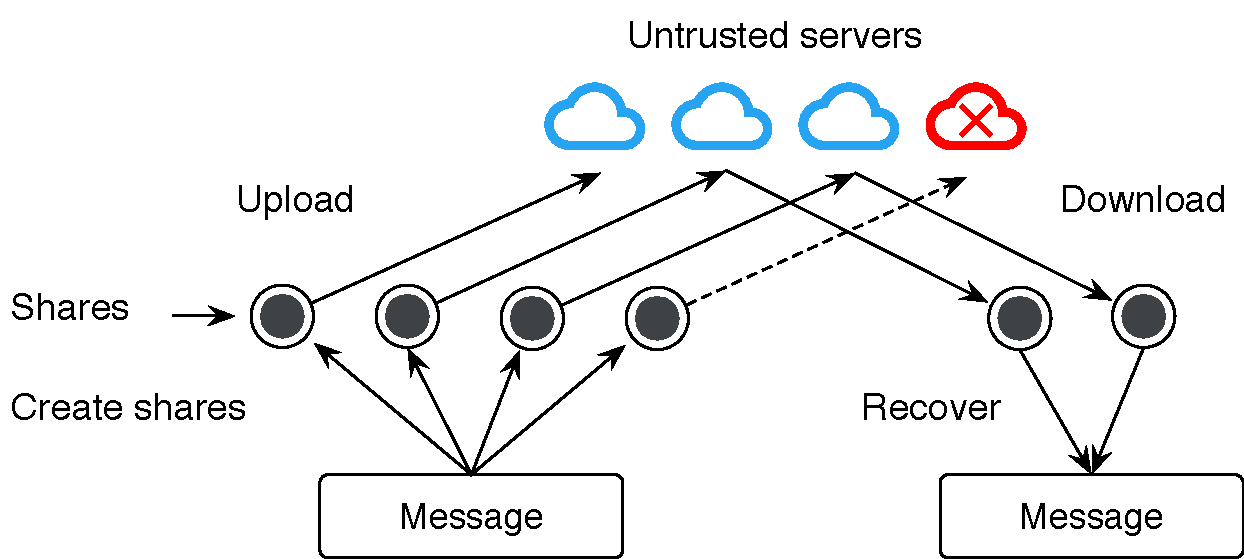
\includegraphics[scale=0.42]{transportation}
	\caption{Message transportation using the extended secret sharing scheme $f(2, 4, 3)$.}
\end{figure}

\subsection{Grouper Message Protocol}

The Grouper API layer sends and receives messages using our own protocol, the Grouper Message Protocol.
In this protocol, a message is a JSON string that contains a marshalled object and its attributes.
Table 3 shows the attributes in a Grouper message.
There are three important attributes:

\begin{itemize}
	\setlength{\itemsep}{1pt}
	\setlength{\parskip}{0pt}
	\setlength{\parsep}{0pt}
	\item \textbf{Type.}
	This attribute refers to the message types.
	There are four types of messages: update messages, delete messages, confirm messages, and resend messages.
	An update message contains the marshalled objects of an application.
	A delete message contains the identifier of a deleted object.
	A confirm message contains the sequence numbers of all normal messages created in a device.
	A resend message contains the sequence numbers of missing messages.
	We call update messages and delete messages \emph{normal messages}. 
	Both confirm messages and resend messages contain control information about a reliable multicast. 
	We call these messages \emph{control messages}.
	\item \textbf{Content.} 
	If the message is an update message, the content value contains the JSON string of a marshalled object.
	If the message is a delete message, the content value contains the objectId of an object.
	If the message is a confirm message, the content value contains the maximum sequence number of messages created in the device of the sender.
	If the message is a resend message, the content value contains the range of missing message sequence numbers.
	\item \textbf{Sequence.}
	This attribute refers to the sequence number of a message.
	When a sender sends a new normal message, the sender increments the sequence number and includes it in the new message.
	The sequence number of any control message is 0.
	Both the sequence number and the ID of the sender are needed to identify a unique message.
\end{itemize}

The receiverId attribute contains the addresses of destination devices.
An address is either a list of device IDs or "*", which signifies multicasting to all devices.

\begin{table}[t]
	\centering
	\small
	\caption{Attributes of the Grouper message.}
	\begin{tabular}{lll}
		\hline
		\textbf{Attribute} & \textbf{Explanation} \\ \hline
		type & Type of this message. \\
		content & A marshalled object or sequence numbers. \\
		sequence & Sequence number of the message. \\
		class & Class name of an object. \\
		objectId & ID of an object. \\
		receiverId & Node identifier of the receiver. \\
		senderId & Node identifier of the sender. \\
		email & Email address of the sender. \\
		name & Name of the sender. \\
		sentTime & Time the message is sent. \\
		\hline
	\end{tabular}
\end{table}

\begin{algorithm}[t]
	\caption{Handle message algorithm}\label{alg:euclid}
	\begin{algorithmic}[1]		
		\Procedure{onMessageReceived}{$msg,\ sender$}
		\LeftComment Check duplicate message.
		\State  $historyMsgs \gets getMsgsBySender(msg.sender)$
		\If{$msg \in historyMsgs$}
		\State \textbf{return}
		\EndIf
		\State $lastMsg \gets historyMsgs.last()$
		\State $historyMsgs.add(msg)$
		
		\LeftComment Basic reliable multicast.
		\If{$ msg.seq \neq  0 \ \&\& \ lastMsg.seq + 1 \neq  msg.seq$}
		\State $resendMsg \gets createResendMsg(lastMsg.seq\ +\ $ \\\hspace{2.7cm} $1,\ msg.seq)$
		
		\Comment Create a resend message with the minimum and \\\hspace{1.7cm} maximum sequence number.
		\State $sendMsg(resendMsg,\ sender)$
		\EndIf
		
		\LeftComment Handle the message by its type.
		\If{$msg.type = "update"$}
		\State $sync.updateRemote(msg)$
		\ElsIf{$msg.type = "delete"$}
		\State $sync.deleteRemote(msg)$
		\ElsIf{$msg.type = "confirm"$}
		\State $maxSeq = getMaxSeqFrom(msg.content)$
		\State $resendMsg \gets createResendMsg(lastMsg.seq\ +\ $ \\\hspace{2.7cm}  $1,\ maxSeq)$
		\If{$resendMsg \neq null $}
		\State $sendMsg(resendMsg,\ sender)$
		\EndIf
		\ElsIf{$msg.type = "resend"$}
		\State $seqs \gets getSeqs(msg.content)$
		\For{$ seq \in seqs$}
		\State $missingMsg \gets getMsg(seq)$
		\State $sendMsg(missingMsg,\ sender)$
		\EndFor
		\EndIf
		\EndProcedure
	\end{algorithmic}
\end{algorithm}

Applications send update, delete and confirm messages through the Grouper API and send resend messages after receiving messages automatically.
When an application invokes the method $grouper.sender.update()$ the Grouper API layer sends an update message that contains the marshalled object to all devices.
When an application invokes the method $grouper.sender.delete()$, the Grouper API layer sends a delete message that contains the ID of the deleted object to all devices. 
When an application invokes the method $grouper.confirm()$, the Grouper API layer sends a confirm message to all devices. 
The confirm message includes the sequence numbers of objects that were recently created in the device.

The method, $grouper.confirm()$, is invoked in the following situations:

\begin{itemize}
	\setlength{\itemsep}{1pt}
	\setlength{\parskip}{0pt}
	\setlength{\parsep}{0pt}
	\item \textbf{Periodically.}
	For example, an application sends a confirm message once during the TTL.
	\item \textbf{When the device is online.} 
	Sometimes, a device is offline and cannot send a confirm message within the TTL.
	Grouper therefore sends a confirm message when the device is online.
\end{itemize}

Algorithm 1 describes the handle process when the Grouper API layer receives a message.
For an update message or a delete message, Grouper invokes the method $sync.updateRemote()$ or $sync.deleteRemote()$ of the synchronization plugin to update the persistent store.
For a confirm message, the Grouper API layer copies the sequence numbers from the message content and removes the sequence numbers that exist in the device.
Next, the Grouper API layer creates a resend message that contains the missing sequence numbers and sends it to the sender of the confirm message.
For resend messages, the Grouper API layer retrieves the sequence numbers from the resend message, finds the corresponding normal messages, and sends them to the sender of the resend message.

\subsection{Group Management}

To manage a group, Grouper provides the following two functions:

\begin{itemize}
	\setlength{\itemsep}{1pt}
	\setlength{\parskip}{0pt}
	\setlength{\parsep}{0pt}
	\item Group Creation.
	\item Member Invitation.
\end{itemize}

A user can create a group, and the creator becomes the owner of the group.  
Before creating a group, the owner prepares his own user information (including his email address and name), multiple untrusted servers, a group ID, and a group name. 
Next, the owner initializes the group on all untrusted servers by submitting his node identifier and the TTL to multiple untrusted servers. 
The node identifier, which represents his device, is generated by Grouper randomly when the application is launched for the first time. 
On each untrusted server, the Web service initializes this new group and returns a master key including the highest privilege to the owner. 
The owner can add other members to an untrusted server according to the master key.

After creating a group, the owner can invite new members to his group. 
To join the group, a new member first prepares his user information at first. 
The owner invites the new member in a face-to-face manner, rather than using central servers. 
At this time, Grouper establishes a connection between the devices using a local safe communication channel like \emph{Multipeer Connectivity}\cite{mc}. 
First, the new member sends usethe r information and a node identifier to the owner. 
The owner saves the user information and node identifier to his device. 
Secondly, the owner registers the new member to the multiple untrusted servers by submitting the node identifier of the new member. 
Third, the untrusted servers return access keys for the new member to the owner. 
Last, the owner sends the access keys, the addresses of the untrusted servers and the list of existing members to the new member. 
After receiving them, the new member can access the untrusted servers with the keys.

\section{Implementation}

\begin{table*}[t]
	\small
	\centering
	\caption{Application lines of code.}
	\label{my-label}
	\begin{tabular}{cccccc}
		\hline
		\textbf{Application} & \textbf{Platform} & \textbf{Lanaguage} & \textbf{Number of Entities} & \textbf{Standalone Application LoC} & \textbf{Increased LoC} \\ \hline
		Account Book & iOS & Objective-C & \multicolumn{1}{r}{5} & \multicolumn{1}{r}{8076} & \multicolumn{1}{r}{190} \\ 
		Test & iOS & Swift & \multicolumn{1}{r}{1} & \multicolumn{1}{r}{621} & \multicolumn{1}{r}{18} \\  \hline 
	\end{tabular}
\end{table*}

Grouper consists of a client framework for developing mobile applications and a Web service running on multiple untrusted servers.
We describe the implementation of the client framework in Section 4.1, the implementation of the Web service in Section 4.2, and the demo applications in Section 4.3.

\subsection{Client Framework}

Grouper's client framework is written in Objective-C, and it supports developing applications on iOS, macOS, watchOS and tvOS.
It makes use of the following frameworks.   

\begin{itemize}
	\setlength{\itemsep}{1pt}
	\setlength{\parskip}{0pt}
	\setlength{\parsep}{0pt}
	\item 
	\textbf{Multipeer Connectivity}\cite{mc}, an official Peer-to-Peer communication framework provided by Apple. 
	Grouper uses it to transfer data between two devices in a face-to-face manner using a wireless LAN or Bluetooth network.
	\item 
	\textbf{Core Data}\cite{coredata}, an official (Object-Relational Mapping) ORM framework provided by Apple.
	Core Data provides generalized and automated solutions to common tasks associated with object life cycles and object graph management, including persistence. 
	Grouper uses it to manage model layer objects. 
	\item 
	\textbf{Sync}\cite{sync}, a synchronization framework for Core Data using JSON.
	Grouper currently uses it in the synchronization plugin.
	\item 
	\textbf{c-SSS}\cite{c-sss}, an implementation of the secret sharing scheme.
	\item 
	\textbf{AFNetworking}\cite{afnetworking}, a networking library in Objective-C. 
	Grouper uses it to invoke the RESTful API provided by our Web services running on multiple untrusted servers. 
\end{itemize}

\subsection{Web Service}

We have chosen to implement own Web service rather than using commercial general cloud storage services like Amazon Simple Storage Service (S3), Google Cloud Storage, or Microsoft Azure Storage for the following reasons:

\begin{itemize}
	\setlength{\itemsep}{1pt}
	\setlength{\parskip}{0pt}
	\setlength{\parsep}{0pt}
	\item The Web service must support on the Grouper Message protocol.
	\item The Web service must delete shares after a prescribed time.
\end{itemize}

Our Web service provides a RESTful API to clients.
It runs on a Tomcat server\cite{tomcat} that is an open-source implementation of the Java Servlet, JavaServer Pages, Java Expression Language, and Java WebSocket technologies. 
We use the Spring MVC\cite{spring}, a Web model-view-controller framework, to create our RESTful API, and Hibernate\cite{hibernate}, an open-source Java ORM framework, to save and operate objects in the Web service. 

Our Web service includes three kinds of entities: the \emph{Group}, \emph{User}, and \emph{Share} entities. 
The \emph{Group} entity saves the group ID, group name, and its owner. 
The \emph{User} entity saves the node identifier of a user, the access key for this user, and the group entity of this user. 
The \emph{Share} entity saves a share generated with the secret sharing scheme, at time when a client uploads the share. 

\subsection{Application}

\begin{figure}[t]
	\centering
	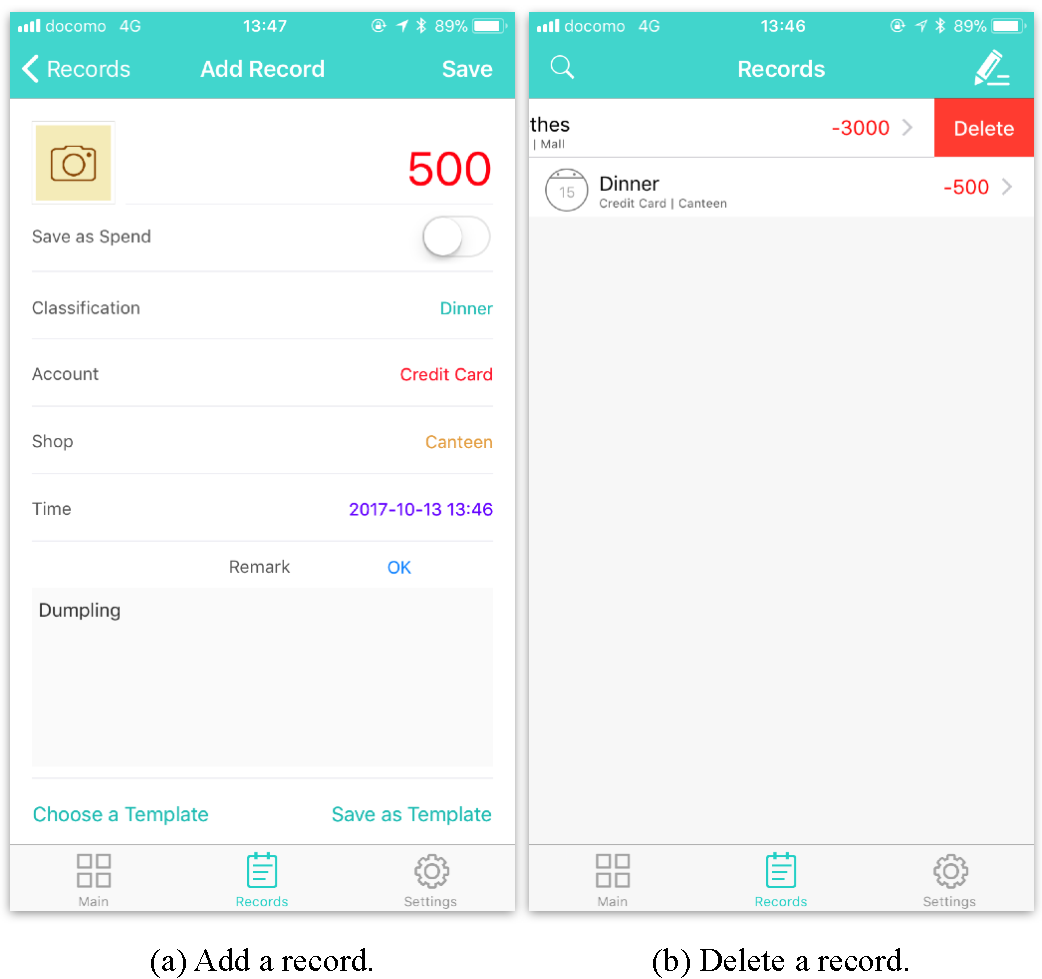
\includegraphics[scale=0.5]{account_book}
	\caption{Screenshots of the Account Book demo application.}
\end{figure}

Using the Grouper framework, we have developed the following applications. 

\begin{itemize}
	\setlength{\itemsep}{1pt}
	\setlength{\parskip}{0pt}
	\setlength{\parsep}{0pt}
	\item \emph{Account Book}, an iOS application in Objective-C, that records the income and expenditure of a group.
	\item \emph{Test}, a benchmark iOS application in Swift, that tests the performance of Grouper.
\end{itemize}

Figure 4(a) shows the screenshot of adding a record in Account Book. 
A user uses Account Book to add income and expenditure records that include the classifications, accounts, shops, times and remarks of a group. 
When the user click the save button, Account Book invokes the $grouper.sender.update(object)$ method of Grouper to share this record with other group members.
Figure 4(b) shows the screenshoot of deleting a record in Account Book. 
A user swipes a cell from right to left to delete a record from the record list. 
When the user click the delete button, Account Book invokes the $grouper.sender.delete(object)$ method of Grouper to delete this record on the devices of other group members.

\begin{figure*}[t]
	\centering
	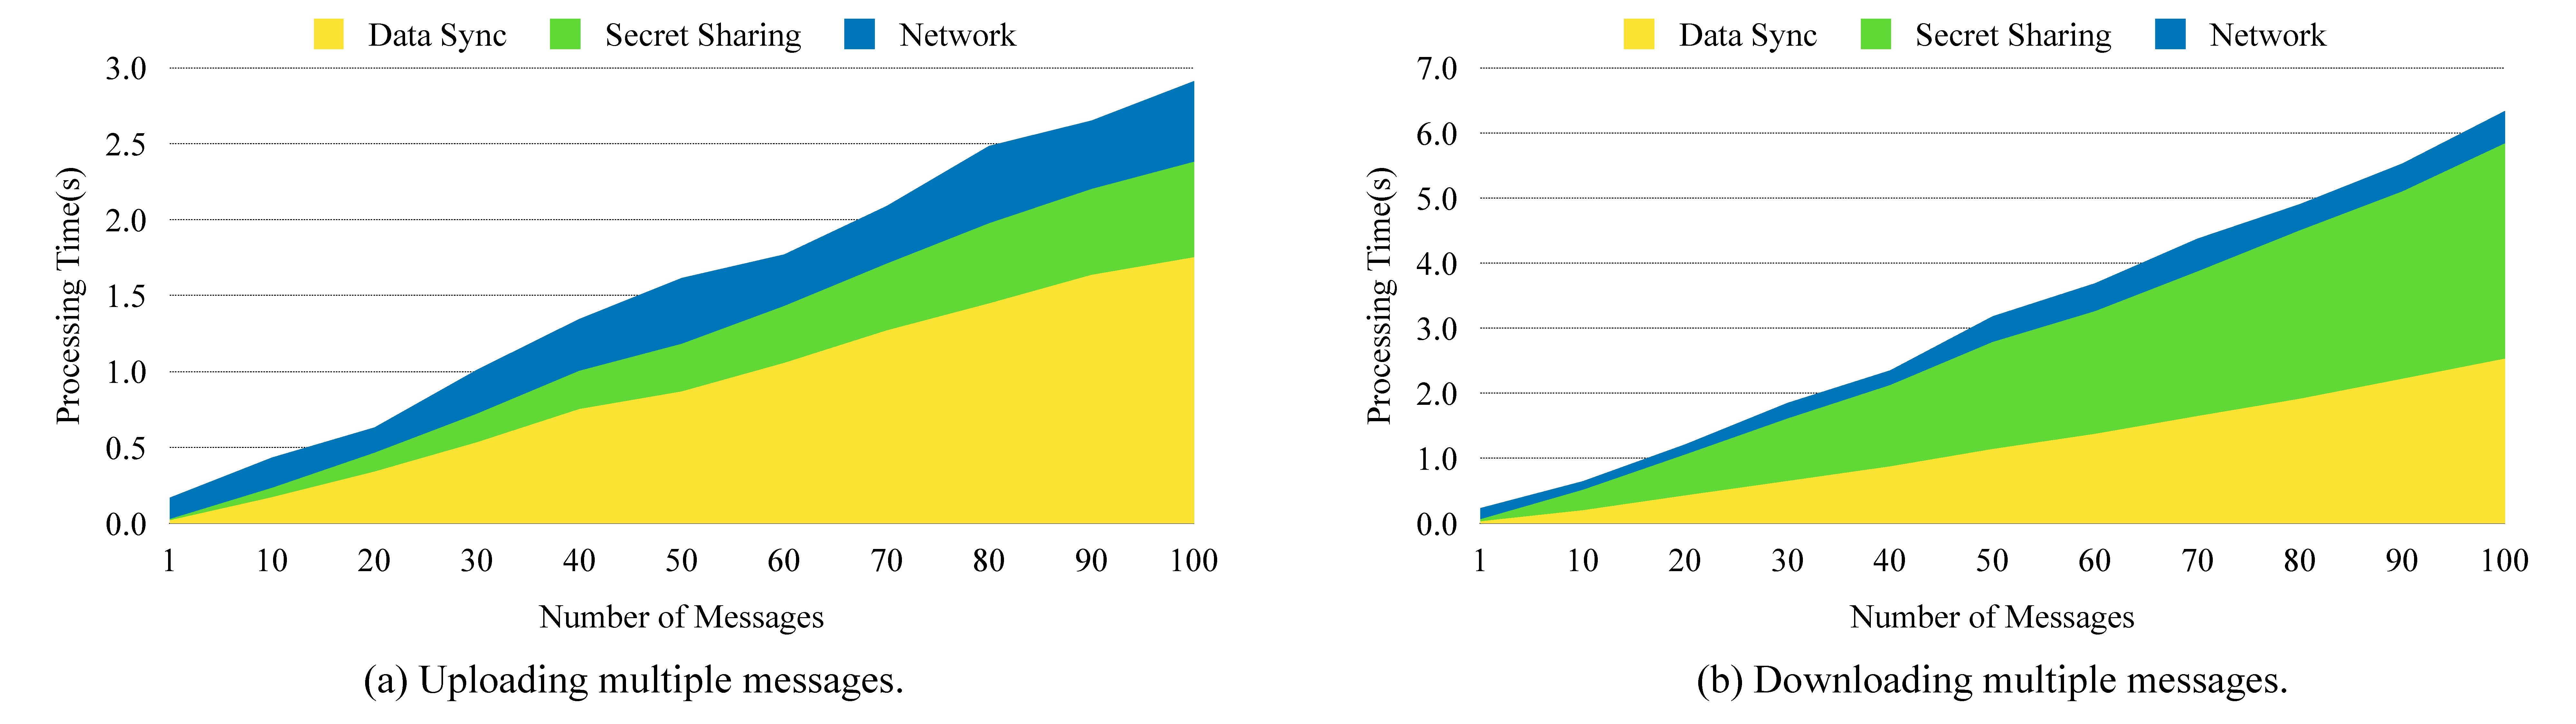
\includegraphics[scale=0.13]{multiple_messages}
	\caption{Processing time of uploading and downloading multiple messages.}
\end{figure*}

\begin{figure*}[t]
	\centering
	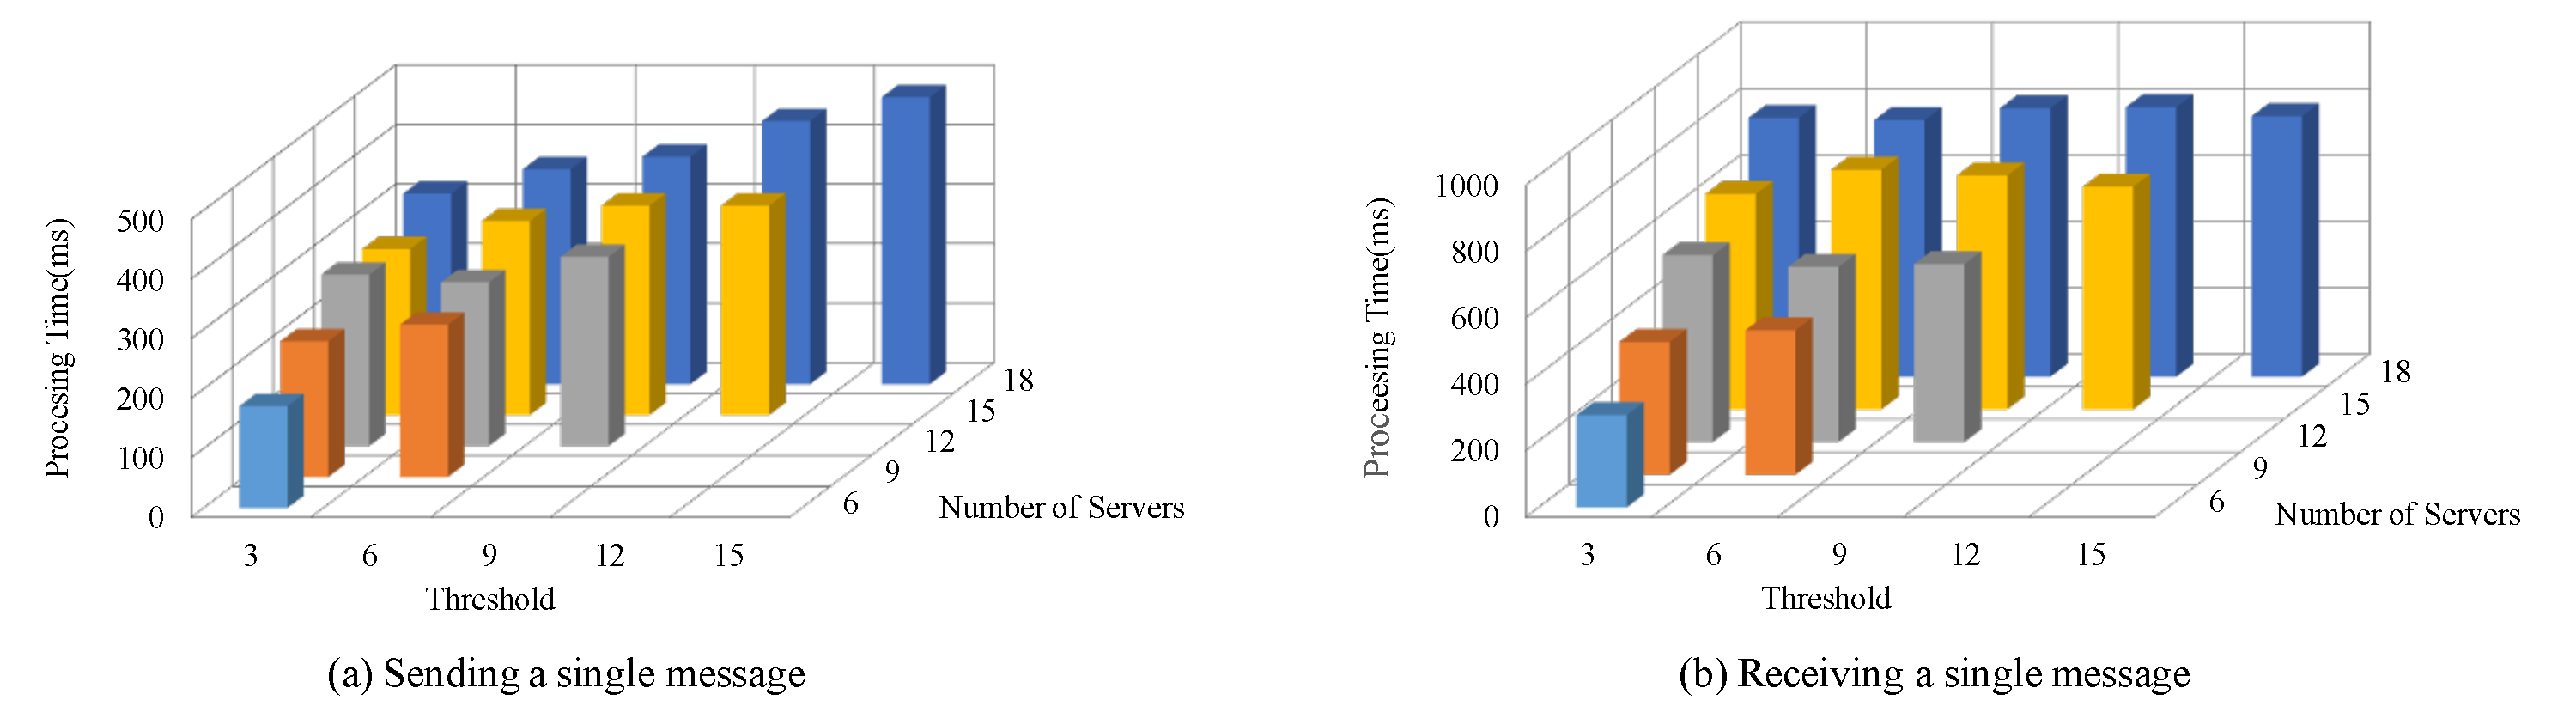
\includegraphics[scale=0.35]{3d}
	\caption{Processing time of uploading and downloading a single message with a different scheme.}
\end{figure*}

\begin{figure*}[t]
	\centering
	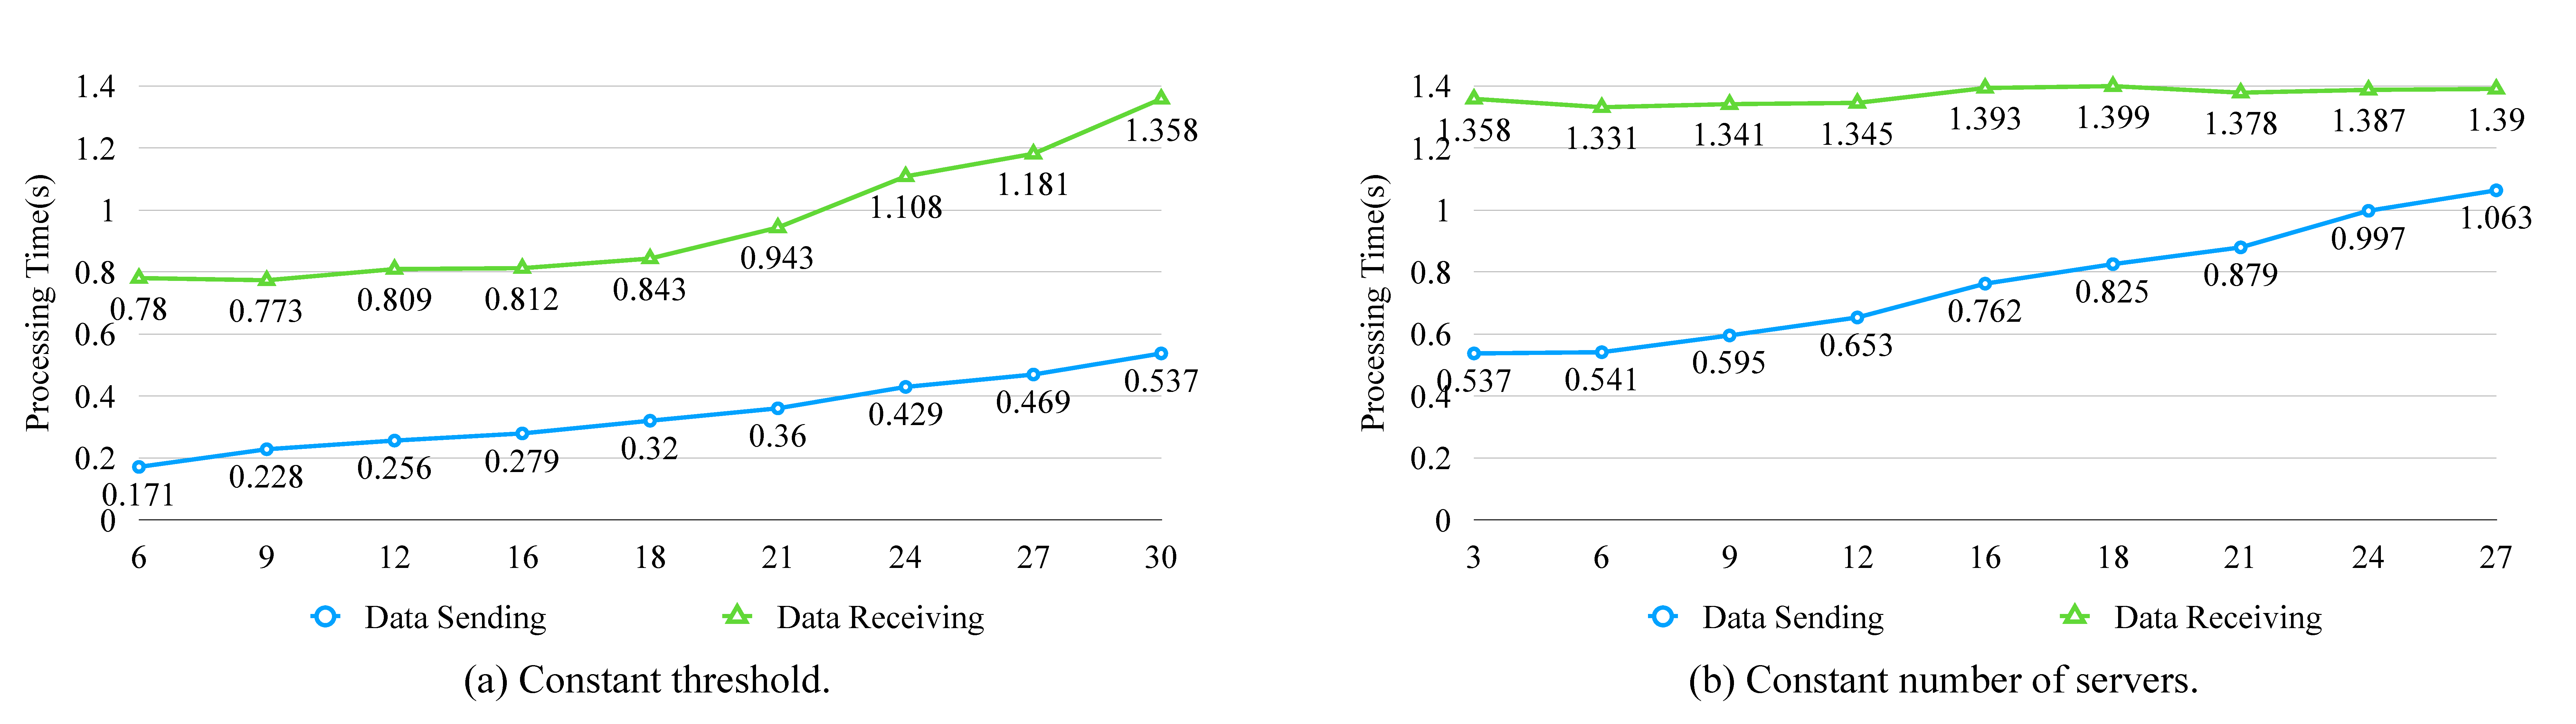
\includegraphics[scale=0.13]{constant_k_n}
	\caption{Processing time of uploading and downloading a single message with a constant ${k}$ or ${n}$.}
\end{figure*}

\section{Evaluation}

This section discusses the development efforts to use Grouper for developing mobile applications, as well as its performance.

\subsection{Development Efforts}

We view the development efforts through two factors: the usability of the client API and the code size, in terms of the lines of code (LoC) the developer has to add after using Grouper. 
As described in Table 1, Grouper provides a simple client APIs for developers.
A developer can easily convert a standalone application to a data sharing application with our client APIs.

Section 4.3 demonstrates the implementation of two applications.
Table 4 shows that developers can add data synchronization to these applications with Grouper by adding a small amount of code. 

The Grouper framework provides the synchronization as a pluggable module.
We use the Sync\cite{sync} framework.
It provides a consistency model where currently, the newest object wins in the synchronization plugin.
For example, if a record in the Account Book application has been modified by two users, the modification of one user will be lost.
Account Book maintains the newest modification and put it into persistent store.

If an application requires another consistency model, the developer has to implement the related synchronization plugin.
For example, if a developer wants to use eventual consistency, he can choose Ensembles\cite{ensembles}.

Note that the synchronization frameworks must provide the interfaces as described in Table 2.
For this reason, Grouper does not support iOS synchronization frameworks for iCloud or Dropbox.
For example, Grouper does not support Core Data with iCloud\cite{coredata} and TICoreDataSync\cite{ticoredatasyn} at this point.
These frameworks provide APIs for files whereas Grouper requires APIs for sending multicast messages.
If a developer want to use them, he has to add an additional layer that provides the methods in Table 2.

\subsection{Performance}

In this subsection, we show that mobile applications using the Grouper framework provide satisfactory performance for small groups of people.
Table 5 lists the hardware and software configuration of our experiment environment.
In our performance experiments, we used the benchmark application \emph{Test} to transfer data between the iPhone 4s and iPod touch 5 generation on a wireless LAN network (802.11n).
We installed 30 Web services on three different servers.
Each server ran a Tomcat server instance which hosted 10 Web services.

In our benchmark application, the size of an object was 323 bytes.
The object corresponded to an income or expenditure record of the Account Book application.
When the object was updated in a node, the Grouper API generated a normal message whose size was 656 bytes.

\begin{table}[t]
	\small
	\centering  
	\caption{Devices in the performance experiment.}
	\begin{tabular}{llll}
		\hline
		\textbf{Device} & \textbf{CPU} & \textbf{RAM} & \textbf{OS} \\ \hline
		iPod 5 & A5 & 512MB & iOS 9.3.5 \\
		iPhone 4s & A5 & 512MB & iOS 9.3.5 \\
		Server 1 & Core i7-5820K & 32GB & Ubuntu 14.04.5 LTS \\
		Server 2 & Core i7-5820K & 32GB & Ubuntu 14.04.5 LTS \\
		Server 3 & Core i7-5820K & 32GB & Ubuntu 14.04.5 LTS \\ \hline
	\end{tabular}
\end{table}

We performed an experiment to measure the processing time of object synchronization according to the number of updated objects.
In this experiment, we set the secret sharing scheme to ${f(2, 3, 3)}$.
We sent multiple messages from a device and received them in another device. 
Concretely, we sent multiple messages from the iPod to the iPhone for three times, and from the iPhone to the iPod for three times.
Then, we obtained the average value of the measured processing times.

Figure 5 shows the processing time of uploading and downloading multiple messages.
We divide the processing time into three parts: data synchronization, secret sharing, and networking.
As the number of messages increased, the data synchronization and secret sharing time increased linearly. 
The networking time increased slowly and sometimes decreased.
On the whole, the total processing time increased linearly.
Compared with uploading messages, downloading messages required about two times more processing time.
Furthermore, object synchronization is done as a background task, asynchronously.
When the Grouper framework is performing object synchronization, the user interface of a mobile application does not freezes.
Therefore, a user is not aware of the occurrence of data synchronization.

We performed an experiment to measure the processing time of object synchronization according to the parameters of the secret sharing scheme.
Specifically, we changed the parameter ${k}$ and ${n}$ of the secret sharing scheme and measured the processing time of uploading and downloading a single message.

Figure 6 shows the relationship between processing time and the parameters, where $s=n,\ 0< k < n,\ k=3i,\ n=3j+3$ and $ 1 \leq i, j \leq 5$.
When uploading a single message, as the parameter ${k}$ or ${n}$ increased, processing time increased linearly.
However, when downloading a single message, as the parameter ${k}$ increased, processing time changed slightly, and sometimes decreased.

Figure 7(a) shows the relationship between processing time and the number of servers ${n}$, where ${k=3}$ and ${n = 2, 4, 6, ... , 10}$.
As $n$ increased, the processing time of uploading and downloading increase linearly. 
Figure 7(b) shows the relationship between processing time and the threshold ${k}$, where ${n=30}$ and ${k = 3, 6, 9, ... , 27}$.
As $k$ increased, the processing time of uploading increased linearly and that of downloading did not change.

\subsection{Discussion on the Number of Messages}

In this subsection, we discuss and the number of messages. 
We use the parameters in Table 6.

\begin{table*}[t]
	\centering
	\small
	\caption{Parameters for discussing the relationship between the TTL and the number of messages.}
	\begin{tabular}{ll}
		\hline
		\textbf{Parameter} & \textbf{Explanation} \\ \hline
		$D$ & Number of devices. \\
		$T$ & Time to live (TTL). \\
		$F$ & Average number of offline devices during the TTL. \\
		$L$ & Average offline time. \\
		$Ui$ & Average number of updated/deleted messages in the device $i$ during the TTL. \\ 
		$URi$ & Average number of updated/deleted messages by resend messages in the device $i$ during the TTL.\\ 
		$C$ & Average number of confirm messages in the device $i$ during the TTL. \\ 
		$U$ & Total number of updated and deleted objects during the TTL. \\ 
		$NUi$ & Number of uploads for device $i$ during the TTL. \\
		$NU$ & Total number of uploads during the TTL. \\
		$NDi$ & Number of downloads for device $i$ during the TTL. \\
		$ND$ & Total number of downloads during the TTL. \\ \hline
	\end{tabular}
\end{table*}

First, we consider the situation in which all devices are online ($F=0$).
In this situation, the number of uploads for the device $i$ are:

\begin{equation}
NUi = Ui + C
\end{equation}

Total number of uploads $NU$ is the sum of $NUi$.

\begin{equation}
NU = \sum_{i = 1}^{D} NUi = U + C \cdot D
\end{equation}

A device does not download the messages that is has uploaded.
To simplify these equations, we assume that the device downloads those messages as well.
Thus, the number of downloads for device $i$, $NDi$, is the equal to the total number of uploads $NU$.

\begin{equation}
NDi = NU = U + C \cdot D
\end{equation}

The total number of downloads $ND$ is the sum of $NDi$.

\begin{equation}
ND = \sum_{i = 1}^{D} NDi = NU \cdot D =  (U + C \cdot D) \cdot D
\end{equation}

Since the current cloud servers scale well according to the number of devices and and messages, we discuss $NUi$ and $UDi$ in this subsection.
Equation 1 shows that for the device $i$ during the TTL, the order of uploading is $O(U)$.
Euqation 3 shows that the order of downloading is $O(U+D)$.
As the number of updated and deleted objects increases, the total numbers of uploads and downloads increases linearly.
As the number of devices increases, the number of confirm messages increases linearly.

Next, we consider the situation in which there are offline devices in a group ($F \neq 0$).
In this situation, offline devices send resend messages when they become online and the devices that have the updated objects will resend the update messages to the offline devices.
To simplify these equations, we assume that all offline devices receive the updated messages after they send resend messages.
For the device $i$, the number of those update messages by the resend message, $URi$, is

\begin{equation}
URi = Ui \cdot \frac{L}{T} \cdot F
\end{equation}

Compared to the situation that $F=0$, in this situation, the number of uploads for the device $i$ includes $URi$.
Thus, we obtain $NUi$, $NU$, $NDi$ and $ND$ where $F \neq 0$.

\begin{equation}
NUi = Ui + C + Ui \cdot \frac{L}{T} \cdot F = Ui \cdot (1 + \frac{L}{T} \cdot F) + C
\end{equation}

\begin{equation}
NU = \sum_{i = 1}^{D} NUi = U \cdot (1 + \frac{L}{T} \cdot F) + C \cdot D
\end{equation}

\begin{equation}
NDi = NU = U \cdot (1 + \frac{L}{T} \cdot F) + C \cdot D
\end{equation}

Equations 6 to 8 show that for the device $i$ during the TTL, the order of uploading is $O(U \cdot \frac{L}{T} \cdot F + C)$, and the order of downloading is $O(U \cdot \frac{L}{T} \cdot F + C \cdot D)$.
As the numbers of updated and deleted objects, the average number of offline devices during the TTL, and the average online time increase, the number of uploads and downloads for a single device increases linearly.

If we use a longer $T$, the numbers of messages, $NUi$ and $NDi$, become smaller.
However, this makes it easier for attackers to attack untrusted servers.

Finally, we consider the following two cases with concrete parameters.
In the last two cases, there are ten users in a small group and everyone has a device.
We set the TTL to one day and a hundred of normal messages are created by the ten users in the group during the TTL.
In addition, a device send only one confirm message during the TTL.

\begin{itemize}
	\setlength{\itemsep}{1pt}
	\setlength{\parskip}{0pt}
	\setlength{\parsep}{0pt}
	\item \textbf{Case 1: $D = 10,\ T = 1 \ day,\ Ui = 100,\ C = 1,\ F = 0$.}
	
	In this case, there are no offline users in the group.
	Each device uploads 101 messages and downloads 1010 messages during the TTL.
	\item \textbf{Case 2: $D = 10,\ T = 1 \ day,\ L = 1 \  day,\ Ui = 100,\ C = 1,\ F = 2$.} 
	
	In this case, there are two offline users in the group and the average offline time is one day.
	Each device uploads 301 messages and downloads 3010 messages during the TTL.
\end{itemize}

\section{Related Works}

Vanish is a self-destruction system\cite{geambasu2009vanish} that uses Distributed Hash Tables(DHTs) as the back-end storage.
Vanish encrypts a message with a new random key, threads the key to shares using a secret sharing scheme, stores these shares in a public DHT, and eliminates the key from the local storage.
The key in Vanish is removed after a certain period of time, and the encrypted message becomes permanently unreadable.
Vanish is implemented with OpenDHT\cite{rhea2005opendht} or VuzeDHT\cite{vuzedht} which is controlled by a single maintainer. 
Thus, it is not very secure against some Sybil attacks\cite{wolchok2010defeating}. 
In addition, the surviving time of the key in Vanish cannot be controlled by the applications. 

To address these issues in Vanish, Zeng et al. proposed SafeVanish\cite{zeng2010safevanish} and SeDas\cite{zeng2012sedas}. 
SafeVanish prevents hopping attacks by extending the length range of key shares while SeDas exploits active storage networks instead of P2P nodes to maintain a divided secret key. By extending SeDas, Zeng's group proposed CloudSky\cite{zeng2015cloudsky}, a controllable data self-destruction system for untrusted cloud storage. 
In CloudSky, a user can control the surviving time of a message.
CloudSky uses Attribute Bases Encryption (ABE) and allows users to define access control policies.

However, these systems are not suitable for developing information sharing applications. 
They are suitable for exchanging immutable messages, whereas our target applications need to modify objects repeatedly after other devices receive the object. 
Although CloudSky solves the problems regarding user controllability that exist in Vanish, offline devices cannot download messages after they have been removed from untrusted servers.
In Grouper, offline devices can download such messages by using confirm and resend messages.
A trusted authority is necessary in CloudSky to manage user profiles, while Grouper does not rely on any trusted authority.

Mylar\cite{popa2014building} stores encrypted data on an untrusted server and decrypts this data only in the browsers of users. 
Application developers of Mylar use its API to encrypt regular (non-encrypted) Web applications. 
Mylar uses its browser extension to decrypt data on the client-side. 
Compared to Mylar, which uses a single untrusted server, Grouper takes advantages of the data redundancy provided by the secret sharing scheme by using multiple untrusted servers.

Sweets\cite{sweets} is a decentralized social networking service (SNS) application that uses data synchronization with P2P connections among mobile devices. 
Sweets performs data synchronization not only between two online nodes directly but also via common friend nodes indirectly for offline nodes.
This indirect synchronization uses ABE to provide access control.
Direct synchronization can only be done when two devices are online at the same time. 
On the other hand, in Grouper, users can synchronize data from multiple untrusted servers, anytime.

DepSky\cite{bessani2013depsky} implements the concept of \emph{Cloud-of-Clouds}.  
DepSky keeps encrypted data in commercial storage services and performs application logic in other individual servers.
In Grouper, untrusted servers undertake the responsibility of temporary data storage and message delivery.
Mobile devices perform application logic.

SPORC\cite{feldman2010sporc} is designed for developing group collaboration applications using untrusted cloud resources.
To maintains synchronization among clients, SPORC uses operational transformation (OT), which allows each client to apply local updates optimistically.
In SPORC, synchronization of nodes should be done online, while Grouper allows for offline synchronization of nodes.

\section{Conclusion}

This paper describes Grouper, a framework using a secret sharing scheme and multiple untrusted servers, to implement light-weight information sharing in mobile applications.
In an application using Grouper, users can create a group and share objects safely via multiple untrusted servers.
Grouper provides two main functions: reliable data synchronization and group management.
Compared to conventional self-destruction systems, Grouper provides the reliable synchronization and allows mobile devices to synchronize data with other devices after untrusted severs remove the data.
Compared to pure data encryption approaches, Grouper improves dependability by using multiple untrusted servers and an extended secret sharing scheme $f(k, n, s)$.

We have implemented Grouper's client's framework in Objective-C and the Web service in Java. 
In addition, we have developed applications, \emph{Account Book} and \emph{Test}, using Grouper.
The development of these applications demonstrate that Grouper requires little development effort to convert an standalone application into a data sharing application.
We also evaluated the performance of Grouper using our benchmark application.
The results shows that using Grouper in an application does not influence user experience.

In the future, we would like to support additional platforms, including Android.
We also have a plan to use file-oriented APIs for exchanging messages among devices.

\begin{acks}
	The authors would like to thank Elvis Nun{\~e}z for helping us to fix some Objective-C related issues of the Sync framework, and Bernard Paulus for fixing a bug of the implementation of the secret sharing scheme, c-SSS.
	
	The authors would also like to thank University of Tsukuba for providing registration fee.
\end{acks}


\bibliographystyle{ACM-Reference-Format}
\bibliography{ref} 

\end{document}
